% Desenvolvimento

\chapter{Planejamento}

\section{Definição da equipe}

Os recursos humanos e seus respectivos papéis 
envolvidos no projeto são definidos na Tabela \ref{tab:recursos} . 

\begin{table}[!htb]
    \begin{center}
        \caption{Recursos Humanos.} \label{tab:recursos}
        \begin{tabular}{ p{4cm} | p{4cm} }
            \hline
            \textbf{Papel} & \textbf{Recurso Humano} \\
            \hline
            Diretor de DW & Ronan Romeu Knob \\
            \hline
            Gerente de projetos de DW & Sabrina Schütz de Oliveira
             \\
            \hline
            Analista de negócios & Giancarlo Souza de Freitas \\
            \hline
            Arquiteto de DW & Giancarlo Souza de Freitas \\
            \hline
            Equipe técnica & Valdir Luiz Hofer Arnhold \\
            \hline
        \end{tabular}
    \end{center}
    Fonte: Os autores (2017).
\end{table}
 
\section{Cronograma}

O projeto de \textit{Data Mart} Ronbuster 
foi pensado para ter início no mês 
de março. Sua duração estimada foi 
estipulada em 6 meses, contemplando as 
fases apresentadas no tabela x. 
A escolha deste período de início foi 
devido a que é o período de término das 
férias escolares, o que deve baixar o movimento 
das filiais, estando pronto também antes do final 
do ano, novo grande ciclo de férias.

Sendo assim, as datas iniciais de início e término do projeto são:

\begin{itemize}
    \item Início do projeto - 01/03/2017;    
    \item Término do projeto - 31/08/2017;    
    \item Dias úteis neste período: 129; e
    \item Horas do projeto: 1032h
\end{itemize}

Abaixo temos uma estimativa das fases do projeto, e seu tempo esperado.
Os valores apresentados não consideram feriados e sábados e domingos. Cálculo da hora é feito por dias úteis * 8h.

\begin{table}[!htb]
    \begin{center}
        \caption{Estimativa de tempo.} \label{tab:tempo}
        \begin{tabular}{ p{3cm} |  p{2.2cm} | p{2.3cm} | p{1.2cm} }
            \hline
            \textbf{Fase} & \textbf{Data de início}  & \textbf{Data de término} & \textbf{Duração} \\
            \hline
            Planejamento do projeto & 01/03/2017 & 24/03/2017 & 144 h \\
            \hline
            Entrevistas &
            27/03/2017 &
            07/04/2017 &
            80 h \\
            \hline
            Definição do esquema estrela e plano de ação &
            10/04/2017 &
            20/04/2017 &
            64 h \\
            \hline        
            Definição da equipe do DW &
            24/04/2017 &
            26/04/2017 &
            24 h \\
            \hline 
            Implementação do DW &
            27/04/2017 &
            09/06/2017 &
            248 h \\
            \hline            
            Criação de portal de dashboards e relatórios &
            12/06/2017 &
            04/08/2017 &
            320 h \\
            \hline 
            Treinamento &
            07/08/2017 &
            11/08/2017 &
            40 h \\
            \hline
            Homologação e ajustes pontuais &
            14/08/2017 &
            31/08/2017 &
            112 h \\
            \hline
            \multicolumn{3}{r|}{Total} & 1032 h \\
            \hline

        \end{tabular}
    \end{center}
    Fonte: Os autores (2017).
\end{table}


\section{Custos}

Com base no Cronograma mostrado e nas horas estimadas o custo projeto é de R\$ 52.000,00.

\chapter{MODELAGEM DIMENSIONAL}

Para a construção do modelo dimensional, 4 passos são necessários, sendo eles:

\begin{enumerate}
\item Decisão de qual processo de negócio deve-se modelar, com base na combinação do conhecimento do negócio com o conhecimento dos dados disponíveis.
\item Definição do grão do processo do negócio, o qual é o nível fundamental atômico de dados que representará o processo na tabela de fatos.
\item Escolha das dimensões que serão aplicadas a cada registro da tabela de fatos.
\item Escolha dos fatos mensuráveis que irão popular cada registro da tabela de fatos.
\end{enumerate}

A seguir, temos a utilização desses passos para a criação da modelagem dimensional em questão, para auxiliar a resolução das perguntas estratégicas levantadas.
 
\section{processo do negócio}

O processo do negócio que será modelado é o movimento diário de item, nos permitindo acompanhar quais filmes estão sendo emprestados, em que lojas, a que preço e em que dias.


\section{Granularidade}

A granularidade, representa o nível de
detalhamento da modelagem.
Para este projeto, se buscou alcançar o maior nível de granularidade possível. Por exemplo, para o 
mapeamento da dimensão do tempo é utilizado a hora, 
dessa forma se torna possível fazer 
consultas por dia ou semanas. 

\section{Dimensões}

As dimensões escolhidas são Tempo, Midia e Loja , conforme mostra a Figura \ref{fig:dimensoes}.  

\begin{figure}[!htb]
   \centering
   \caption{Dimensões.}\label{fig:dimensoes} 
   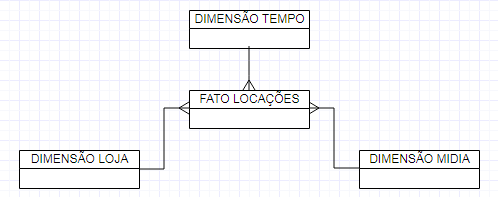
\includegraphics[scale=0.7]{imagens/img1.png}
\end{figure}

\section{Fatos}

Inicialmente foi modelada a seguinte a tabela de fatos de Locações, conforme mostra a Figura \ref{fig:fato0}.


\begin{figure}[!htb]
   \centering
   \caption{Fato - Versão 1.}\label{fig:fato0} 
   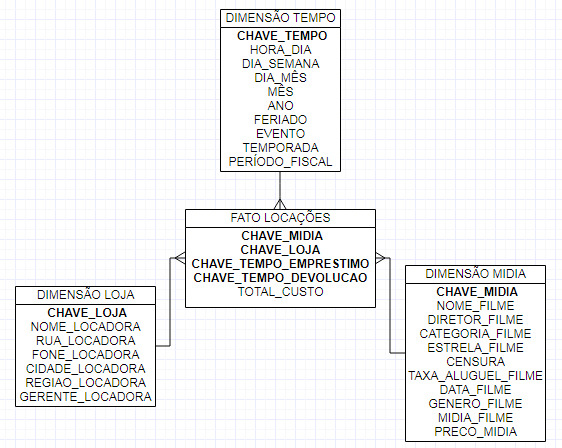
\includegraphics[scale=0.5]{imagens/fato-0.jpeg}
\end{figure}

"Há somente uma garantia para qualquer projeto de DW 
e é a que ele será mudado.” Depois de analisarmos 
novamente a modelagem, e com as perguntas estratégicas 
em mente, percebemos que uma nova tabela fato deveria ser 
adicionada para a resolução dessas perguntas, conforme é mostrado na Figura
 \ref{fig:fato}. 

\begin{figure}[!htb]
   \centering
   \caption{Fato - Versão 2.}\label{fig:fato} 
   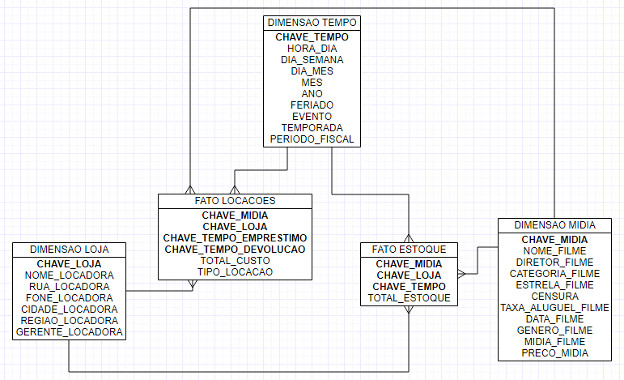
\includegraphics[scale=0.5]{imagens/fato-1.jpeg}
\end{figure}

 
\chapter{Indicadores}

Para verificar se as perguntas estratégicas 
levantadas no projeto da locadora Ronbuster 
estão sendo respondidas, é necessário criar indicadores. 
Os indicadores visam monitorar as variáveis necessárias para 
solucionar uma pergunta estratégica, e criando informação a partir 
delas, que responde aos questionamentos da gestão da empresa. 
Os indicadores são chamados indicadores estratégicos, que são os 
indicadores que podem dar ampla visão dos objetivos e metas mais 
gerais da empresa, bem como permitir a comparação de ações anteriores 
com resultados atuais. 

Quanto a locadora Ronbuster, para responder as perguntas que criamos, 
foram levantados os indicadores mostrados na Tabela \ref{tab:indi} e as 
variáveis mostradas na Tabela \ref{tab:variaveis}.

\begin{table}[!htb]
    \begin{center}
        \caption{Indicadores.} \label{tab:indi}
        \begin{tabular}{ p{4.5cm} |  p{4.5cm}   }
            \hline
            \textbf{Pergunta} & \textbf{Indicador}   \\
            \hline
            Em quanto tempo uma mídia física se paga? & (V1*v4) / (V2*V3) \\
            \hline
            Qual é o fluxo de empréstimos e devoluções das mídias por dia da semana? & (V5*24) e (V5*24)  \\
            \hline
           Qual o número ideal de cópias de cada título por filial? & V7 \\
            \hline

        \end{tabular}
    \end{center}
    Fonte: Os autores (2017).
\end{table}


\begin{table}[!htb]
    \begin{center}
        \caption{Variáveis.} \label{tab:variaveis}
        \begin{tabular}{ p{8cm}    }
            \hline
              V1 - Valor da locação de uma mídia \\
            \hline
              V2 - Custo da mídia (custo de compra de uma unidade) \\
            \hline
            V3 - Quantidade de mídias compradas   \\
            \hline
           V4 - Número de locações de uma mídia \\
            \hline
             V5 - Número de locações por hora \\
            \hline
             V6 - Número de devoluções por hora \\
            \hline
            V7 - Número de títulos disponíveis por hora do título \\
        \hline
        \end{tabular}
    \end{center}
    Fonte: Os autores (2017).
\end{table}

\section{Exemplos de relatórios}

\subsection{Pergunta 1}

A consulta para responder a pergunta 1, 
pode ser como acima. Nela, é apresentado o 
título da mídia, preço desta. Para resolver 
quanto tempo, foi calculado a média do custo da locação, 
considerando que pode haver diferença de custo por algum motivo, 
dividido pela média de dias que ela esteve locada. Considerando 
então uma locação de 24h, ou seja,1 locação por dia, temos, dividindo 
o preço por esta média, o número de dias em que a mídia se pagará.

\begin{figure}[!htb]
   \centering
   \caption{Resposta da pergunta 1.}\label{fig:fato} 
   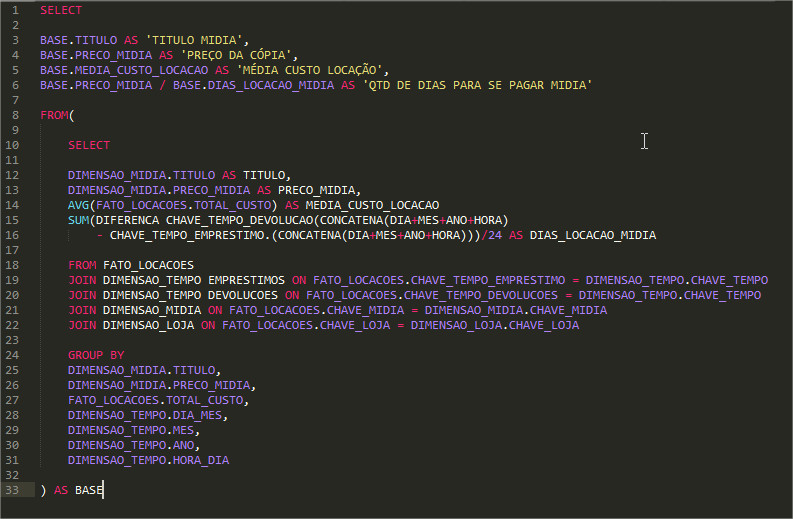
\includegraphics[scale=0.4]{imagens/sql-1.jpeg}
\end{figure}

As funções de diferença de tempo e concatenação de 
campos para formar as datas foram omitidas por apresentarem 
peculiaridades técnicas pertencentes a cada SGBD.

\subsection{Pergunta 2}

Para a pergunta estratégica 2: Qual é o fluxo de empréstimos e devoluções das mídias por dia da semana?

\begin{figure}[!htb]
   \centering
   \caption{Resposta da pergunta 2.}\label{fig:fato} 
   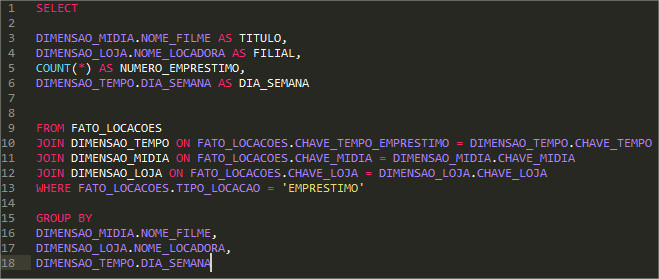
\includegraphics[scale=0.5]{imagens/sql-0.jpeg}
\end{figure}

Essa pesquisa retorna os dias da semana e a quantidade 
de cópias emprestadas, separados por título  e filial. 
A agregação poderia ser por qualquer unidade de tempo. 
Para saber a quantidade de devoluções, como a pergunta 2 
também exige, precisaria apenas mudar, na linha 13, a palavra 
\textbf{'EMPRESTIMO'} para \textbf{'DEVOLUCAO'}, e a chave da tabela 
de \textbf{'FATO\_LOCACOES'} para 
\textbf{'CHAVE\_TEMPO\_DEVOLUCAO'} .

